\chapter{静态有向模型}
\label{chap:pgm-static-directed}

同一台设备的两个传感器经常同时给出较高读数。描述这种相关性至少有两种办法：直接用第一个读数预测第二个读数，或假设二者受到某个未观测工作状态的共同影响。两种办法都能定义观测数据的联合分布，却把计算放在不同位置。前者需要拟合条件分布；后者还需要回答工作状态是什么，以及怎样把这个状态从联合分布中消去。一个模型能否解释相关性、能否评价似然、能否补全缺失观测，并不是同一个问题。

第~\ref{chap:pgm-directed}章已经建立有向分解的概率语义，前面的推断与学习章节也给出了处理求和、积分和未知参数的通用方法。本章把这些工具落实到静态模型中。“静态”表示这里不假设变量沿真实时间演化，不表示变量之间没有依赖。记一条记录的观测为$\bm{x}\in\mathbb{R}^d$或相应的离散取值向量，训练集包含$n$条记录$\bm{x}_1,\ldots,\bm{x}_n$，全部待估计参数合记为$\bm{\theta}$。类别标签存在时另记为$Y$，此时完整图还包含类别节点。

本章围绕“怎样用有向结构定义并使用观测分布”展开。直接模型从观测之间建立条件分布；潜变量模型则先定义更大的联合分布，再求和或积分得到观测分布。潜变量可以离散，也可以连续；它们还可以在多个组之间共享，或允许同一组同时使用多个成分。取值类型和共享方式描述不同的属性，不能排成互斥类别。模型比较将回到这两组属性，说明它们如何影响推断、参数估计和结果解释。

\section{直接模型}
\label{sec:pgm-static-directed-direct}

当一条完整记录给出了图中所有随机变量的取值时，有向分解可以直接评价这条记录的概率。只要每个局部条件分布已归一化且可计算，联合分布就不需要另求全局归一化常数。不过，完整记录的概率容易计算，不保证任意缺失模式下的边缘概率同样容易计算。下面的两个模型族分别通过限制父集、共享条件分布的计算来控制规模。

\subsection{朴素贝叶斯与树增强模型}
\label{sec:pgm-static-directed-naive-tan}

若训练记录既有传感器读数又有设备类别，可以先按类别描述读数的分布，再反推新设备的类别。\term{朴素贝叶斯}（naive Bayes, NB）把类别作为所有属性的共同父节点：给定类别后，各属性分别生成，不再相互提供信息。设$Y$有$K$个类别，其概率为$\pi_k=p(Y=k)$，则
\begin{equation}
  \label{eq:pgm-static-directed-naive}
  p(y,\bm{x})=\pi_y\prod_{i=1}^{d}p(x_i\mid y),\qquad
  p(y\mid\bm{x})=
  \frac{\pi_y\prod_i p(x_i\mid y)}
       {\sum_{k=1}^{K}\pi_k\prod_i p(x_i\mid k)}.
\end{equation}
这里的条件独立是给定类别后的共同独立，而不只是属性之间两两独立。把$Y$消去以后，各属性通常仍然相关。训练时类别与属性均已观测，所以最大似然估计分解为类别比例与每类内的局部估计；预测时类别未知，但只需枚举$K$个类别。变量在当前查询中是否已知取决于给定的证据；预测时尚未知晓的标签不因此成为模型主动引入的潜变量，也不等于本应记录却漏记的缺失值。

对二值属性，可用$a_{i,k}=p(X_i=1\mid Y=k)$参数化。若训练集中类别$k$的样本数为$n_k>0$，其中第$i$个属性取$1$的次数为$n_{i,k}^{+}$，则$\widehat\pi_k=n_k/n$、$\widehat a_{i,k}=n_{i,k}^{+}/n_k$。零计数可能把测试记录的整个乘积压成零；采用正的Dirichlet伪计数可以平滑条件表。未出现过的类别或父配置需要先验或额外约束，不能直接计算$0/0$。连续属性也可使用类内高斯密度等局部模型，但仍需明确其分布假设。

以二分类为例，若所有$a_{i,k}$与类别先验都严格位于$(0,1)$，对数后验比为
\begin{equation}
  \label{eq:pgm-static-directed-naive-boundary}
  \begin{aligned}
  \log\frac{p(Y=1\mid\bm{x})}{p(Y=0\mid\bm{x})}
    &=b+\sum_{i=1}^{d}w_i x_i,\\
  b&=\log\frac{\pi_1}{\pi_0}
       +\sum_i\log\frac{1-a_{i,1}}{1-a_{i,0}},\\
  w_i&=\log\frac{a_{i,1}(1-a_{i,0})}
                       {a_{i,0}(1-a_{i,1})}.
  \end{aligned}
\end{equation}
这个线性边界来自伯努利对数似然比，不是“所有朴素贝叶斯都线性”的结论。类间方差不同的高斯属性会产生平方项；一般类别属性则可以看成对类别指示特征的加性评分。生成式估计得到这些系数的方式，也不同于直接最小化分类损失。

\begin{example}[两个二值读数]
  \label{ex:pgm-static-directed-binary}
  为比较直接分解与潜变量解释，另设一个人工传感器模型，不把它看作四节点报警模型的改名。$Y=1$表示某种异常工作状态，$X_1,X_2$是两个二值读数。设
  \[
  \begin{gathered}
    p(Y=1)=0.1,\\
    p(X_1=1\mid Y=1)=0.8,\quad
    p(X_1=1\mid Y=0)=0.1,\\
    p(X_2=1\mid Y=1)=0.7,\quad
    p(X_2=1\mid Y=0)=0.2.
  \end{gathered}
  \]
  在给定$Y$时假设两个读数独立。观测到$(X_1,X_2)=(1,1)$后，两类的未归一化概率分别为$0.1\times0.8\times0.7=0.056$和$0.9\times0.1\times0.2=0.018$，所以
  \[
    p(Y=1\mid1,1)=\frac{0.056}{0.074}
      =\frac{28}{37}\approx0.7568.
  \]
  边缘上$p(X_1=1)=0.17$、$p(X_2=1)=0.25$，而$p(1,1)=0.074$不等于$0.17\times0.25=0.0425$。二者的协方差为$0.0315$：共同类别足以产生观测相关性。
\end{example}

条件独立假设失效时，多个读数可能重复贡献同一份证据。在另一个极端情形中，令$X_2=X_1$为完全相同的复制读数，保留上例的类别先验与$X_1$分布。正确后验为$0.08/(0.08+0.09)=8/17$；误当作两个独立属性后，后验变成$0.064/(0.064+0.009)=64/73$。类别判断甚至会改变，且预测置信度被明显放大。分类准确率较好也不能单独证明独立性假设或后验概率校准良好。

要保留容易学习的结构，同时允许属性之间有一些类内相关性，可以使用\term{树增强朴素贝叶斯}（tree-augmented naive Bayes, TAN）：类别仍指向所有属性，属性之间再增加一棵树。选一个属性$r$为树根，把树边从根向外定向；非根属性$i$的属性父节点记为$t(i)$，则
\begin{equation}
  \label{eq:pgm-static-directed-tan}
  p(y,\bm{x})=
    p(y)p(x_r\mid y)
    \prod_{i\ne r}p(x_i\mid y,x_{t(i)}).
\end{equation}
每个属性最多增加一个属性父节点。给定类别后，图变成一棵有向树，而不再是相互独立的节点。图~\ref{fig:pgm-static-directed-classifiers}画出了这项变化；树边表示允许利用类内依赖，并不自动具有因果含义。

\begin{figure}[htbp]
  \centering
  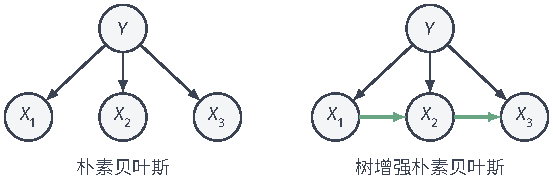
\includegraphics[width=\linewidth]{figures/03-models/03-probabilistic-graphical-models/tikz/pgm-static-directed-classifiers/figure.pdf}
  \caption{朴素贝叶斯与树增强模型。两图的类别$Y$均指向三个属性；右图增加$X_1\to X_2\to X_3$，因此给定$Y$后仍保留树上的属性依赖。节点是否观测由训练或预测任务决定。}
  \label{fig:pgm-static-directed-classifiers}
\end{figure}

结构增加多少参数，可以直接数条件表的自由度。设属性$i$有$r_i$种取值，NB需要$(K-1)+K\sum_i(r_i-1)$个自由参数；固定一棵TAN树后，需要
\[
  (K-1)+K(r_r-1)
       +K\sum_{i\ne r}r_{t(i)}(r_i-1).
\]
两个类别、三个二值属性时，参数数目从$7$增加到$11$。这远小于不受限制的完整联合表，但每个新条件表需要更多样本支持。对完整记录，两种模型的类别评分都只需$O(Kd)$次局部查询；二值TAN的对数评分可包含$x_i x_{t(i)}$交互项，因而不局限于NB的加性边界。

TAN的树可以从完整离散训练数据中求得。用经验分布$\widehat p$定义条件互信息
\[
  \widehat I(X_i;X_j\mid Y)=
  \sum_{y,x_i,x_j}\widehat p(y,x_i,x_j)
  \log\frac{\widehat p(x_i,x_j\mid y)}
                 {\widehat p(x_i\mid y)\widehat p(x_j\mid y)}.
\]
对正频数项计算此式，零频数项按连续延拓取$0$。把任意候选树的条件表取为最大似然估计，平均训练对数似然就等于
\begin{equation}
  \label{eq:pgm-static-directed-tan-score}
  -\widehat H(Y)-\sum_i\widehat H(X_i\mid Y)
  +\sum_{\{i,j\}\in E_{\mathrm{T}}}
       \widehat I(X_i;X_j\mid Y),
\end{equation}
其中$\widehat H$为经验熵，$E_{\mathrm{T}}$为属性树的无向边集。等式来自每条树边上的恒等式$H(X_i\mid Y,X_j)=H(X_i\mid Y)-I(X_i;X_j\mid Y)$；根节点保留原来的条件熵，其余节点各贡献一条边的互信息。前两项不依赖树，因此用条件互信息作边权求最大生成树即可，再任取根定向。无惩罚、观测完整、自由条件表是这个结论的前提；加入结构惩罚或参数约束后不能直接照搬。

若所有$r_i\le r$，朴素的成对计数需要$O(nd^2)$次更新，遍历条件表计算边权需要$O(Kd^2r^2)$操作，稠密图上的最大生成树可在$O(d^2)$时间内得到。NB无需搜索树，计数只需$O(nd)$次更新。TAN用这项额外结构学习成本换取类内依赖，却不能表示任意高阶相互作用；稀疏数据下，一条虚假的树边也会增加估计误差。TAN的提出与具体算法见Friedman等人的工作，树结构学习的一般推导可回看第~\ref{chap:pgm-structure-learning}章\scite{pgm-static-directed-friedman1997}

\subsection{自回归密度模型}
\label{sec:pgm-static-directed-autoregressive}

如果目标是拟合观测分布，而不是依赖某个已知类别来简化属性关系，可以为每个变量保留全部前驱。选定顺序后，将排在第$i$位之前的取值向量记为$\bm{x}_{<i}$。\term{自回归密度模型}（autoregressive density model）逐个预测当前变量的条件分布，再把这些条件分布相乘：
\begin{equation}
  \label{eq:pgm-static-directed-ar}
  p_{\bm{\theta}}(\bm{x})
    =\prod_{i=1}^{d}p_{\bm{\theta}}(x_i\mid\bm{x}_{<i}).
\end{equation}
这里的顺序可以是表格字段顺序或图像像素的扫描顺序，不一定是真实时间；$\bm{x}_{<1}$为空，第一项就是边缘分布。

式~\eqref{eq:pgm-static-directed-ar}为何自动归一化？在离散情形，先对$x_d$求和，最后一个条件分布的和为$1$；再对$x_{d-1}$求和，如此递推，最终剩下$\sum_{x_1}p(x_1)=1$。连续情形把求和改为积分，对非负、可测且对每个前缀归一化的条件密度，可由Tonelli定理交换积分顺序，得到同一结论。由给定联合分布反求条件分布时，零概率前缀上的条件分布可以任意补成归一化分布，不会改变原联合分布。这证明的是模型的归一化，不是它已经拟合真实数据。

链式法则本身对表达能力没有限制：任意给定联合分布都可以沿任意排列写成这种形式。限制来自局部参数化。若每个二值条件都用完整条件表，参数总数仍为$1+2+\cdots+2^{d-1}=2^d-1$；换成有限宽度的网络、有限感受野或简单高斯条件后，不同顺序就可能对应不同难度和不同近似误差。某个顺序使条件分布接近单峰，反向顺序的条件分布却可能多峰；小容量模型不会自动适应这种变化。

例~\ref{ex:pgm-static-directed-binary}的两个读数也能直接自回归建模。把类别求和消去后，得到观测分布
\[
  \begin{array}{ccccc}
    (x_1,x_2)&(0,0)&(0,1)&(1,0)&(1,1)\\
    p(x_1,x_2)&0.654&0.176&0.096&0.074
  \end{array}
\]
相应的三个自回归参数为
\[
  \begin{aligned}
    p(X_1=1)&=0.17,\\
    p(X_2=1\mid X_1=1)&=\frac{37}{85},\\
    p(X_2=1\mid X_1=0)&=\frac{88}{415}.
  \end{aligned}
\]
例如$p(1,1)=0.17\times37/85=0.074$。这个直接分解完整保留了读数之间的相关性，但没有给出工作状态$Y$的含义与后验。观测分布相同，不等于模型对未观测机制作出了同样的解释。

为减少条件表的规模，\term{神经自回归分布估计器}（neural autoregressive distribution estimator, NADE）在不同前缀之间共享神经网络参数。对二值观测，一个宽度为$h$的单隐藏层形式为
\begin{equation}
  \label{eq:pgm-static-directed-nade}
  \begin{aligned}
    \bm{a}_i&=\bm{c}+\sum_{j<i}\bm{W}_{:,j}x_j,&
    \bm{h}_i&=\operatorname{sigmoid}(\bm{a}_i),\\
    p(X_i=1\mid\bm{x}_{<i})
      &=\operatorname{sigmoid}
        (b_i+\bm{V}_{i,:}\bm{h}_i).
  \end{aligned}
\end{equation}
其中$\bm{W}\in\mathbb{R}^{h\times d}$、$\bm{V}\in\mathbb{R}^{d\times h}$，$\bm{c}$和$\bm{b}$为偏置，$\operatorname{sigmoid}(u)=(1+\exp(-u))^{-1}$。递推$\bm{a}_{i+1}=\bm{a}_i+\bm{W}_{:,i}x_i$只需$O(h)$操作，整条记录的密度评价因此为$O(dh)$，无需为每个前缀重做全部输入求和。这里的$\bm{h}_i$是输入的确定性函数，不是需要积分的随机潜变量。NADE的共享计算正是其可计算似然的重要来源\scite{larochelle2011}

前缀递推也可以改成一次带约束的前馈计算。\term{掩码自编码分布估计器}（masked autoencoder for distribution estimation, MADE）把违反顺序的网络连接设为零，使第$i$个输出只能读到$\bm{x}_{<i}$。设输入$j$的次序号为$j$，隐藏单元$u$的次序号为$m(u)$。输入到隐藏层只允许$j\le m(u)$的边，隐藏层到输出$i$只允许$m(u)<i$的边。深层网络的中间边要求次序号非递减，输出边仍严格小于$i$；于是任何输入到输出的路径都满足$j<i$，当前变量和未来变量无法泄漏到该条件分布中。

图~\ref{fig:pgm-static-directed-mask}给出三个输入、两个隐藏单元的例子，隐藏次序号为$1,2$。按“行是接收端、列是发送端”排列，两个掩码是
\[
  \bm{M}_{\mathrm{in}}=
  \begin{pmatrix}1&0&0\\1&1&0\end{pmatrix},\qquad
  \bm{M}_{\mathrm{out}}=
  \begin{pmatrix}0&0\\1&0\\1&1\end{pmatrix}.
\]
它们的乘积为$\left(\begin{smallmatrix}0&0&0\\1&0&0\\2&1&0\end{smallmatrix}\right)$，严格下三角；其中$2$表示两条合法计算路径，不表示两倍概率。第一个输出只使用偏置，第三个输入不参与任何条件参数的计算，但它仍作为第三个条件分布的目标取值进入似然。普通自编码器可以直接复制当前输入，因此普通重构误差并不自动成为归一化联合分布的负对数似然；MADE需要上述路径约束\scite{pgm-static-directed-germain2015}

\begin{figure}[htbp]
  \centering
  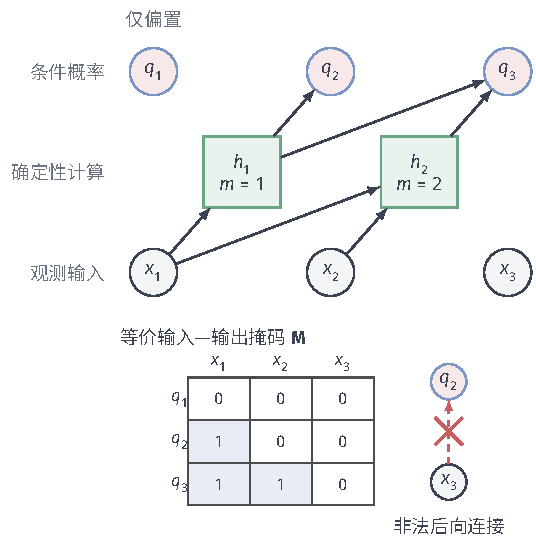
\includegraphics[width=\linewidth]{figures/03-models/03-probabilistic-graphical-models/tikz/pgm-static-directed-mask/figure.pdf}
  \caption{MADE的合法计算路径。方框表示确定性隐藏计算，圆框表示输入或条件分布输出；输出$q_i$代表$p(X_i=1\mid\bm{x}_{<i})$。下方$3\times3$输入—输出掩码直接列出可读关系，蓝格中的1表示允许依赖；右侧以$x_3\to q_2$为非法后向连接反例。隐藏单元的次序号限定可读前缀，任何$q_i$都不能访问$x_i$或更后的输入。}
  \label{fig:pgm-static-directed-mask}
\end{figure}

图像中的条件分布可以利用空间参数共享。\term{像素卷积自回归模型}（PixelCNN）用带掩码的卷积预测各像素的条件分布：按逐行顺序，当前像素只读取上方以及同一行左侧的合法上下文。输入层的掩码排除当前目标；后续隐藏层可以读取当前位置已经合法的隐藏表示，但不能重新接入当前目标值。彩色图像还需约定同一像素内的通道顺序，例如红、绿、蓝，否则通道间也会泄漏目标。有限层数与卷积核形成有限感受野，归一化并不保证网络利用了全部前驱。PixelCNN与PixelRNN在原始论文中共同讨论，本节所用的是卷积掩码这一依赖保证\scite{pgm-static-directed-oord2016}

模型输出的必须是一个分布，而不只是预测均值。二值变量可输出伯努利概率；有$r$种取值的变量可输出经softmax归一化的$r$个概率，原始PixelCNN用这种方式建模每通道$256$个离散值。连续变量则可以输出$\mu_i(\bm{x}_{<i})$与严格为正的尺度$\sigma_i(\bm{x}_{<i})$，得到条件高斯密度；多峰条件可以输出有限高斯混合的权重、均值和尺度。这样的局部混合可以引入一个被显式求和的成分指示变量，所以“使用混合参数化”与“联合似然难算”并不等价。离散概率质量不能直接同连续密度值比较；将量化像素视为连续数据时，还须明确量化区间的积分或去量化方案。

对完整训练数据，负对数似然为
\begin{equation}
  \label{eq:pgm-static-directed-ar-loss}
  L(\bm{\theta})=-\sum_{j=1}^{n}\sum_{i=1}^{d}
      \log p_{\bm{\theta}}
      (x_{j,i}\mid\bm{x}_{j,<i}).
\end{equation}
所有真实前缀已知，MADE和PixelCNN可以在固定网络深度的一次前向计算中同时产生各位置的条件参数，梯度按式~\eqref{eq:pgm-static-directed-ar-loss}求和后更新共享权重。NADE的传统实现利用前缀递推，共享参数也不等于每个条件可以独立训练。训练时应防止额外的跨位置操作破坏掩码，例如未经约束地汇总全部输入后再广播给所有输出。

生成新记录时，未来前缀还不存在。必须先采样$X_1$，再用其结果采样$X_2$，依此进行祖先采样。对具有完整顺序依赖的标量自回归模型，需要$d$轮相继决策；不同样本可以批量生成，但同一样本内部通常不能一次得到所有随机取值。缓存可以减少重复运算，不能消除模型规定的数据依赖。NB的属性在给定类别后反而可以并行生成，TAN也可以按树层并行，因此“有向”本身不是逐变量串行的充分理由。

直接分解的优势是完整似然可算、采样路径明确，但它没有解决所有推断问题。若仅观测一个前缀，剩余变量可以按原顺序生成；若第一维缺失而许多后续维已知，计算该缺失量的条件分布往往需要对一批变量求和或积分。密度评价、祖先生成和任意条件补全的计算难度必须分别判断。第~\ref{chap:pgm-generative}章比较神经参数化生成模型时，将以这里的自回归模型作为直接似然路线的参照。

\section{潜变量模型}
\label{sec:pgm-static-directed-latent}

观测之间的条件分布可以准确预测，却未必提供适合聚类、压缩或组间共享的表示。如果要用一个不可直接观测的状态解释多项观测，就需要把这个状态纳入概率模型。沿用第~\ref{sec:pgm-parameter-learning-definition}节的约定，\term{潜变量}（latent variable）是模型为了表达未观测状态而主动引入的随机量，不是本应记录却未取得的字段值；学习和预测需要处理对它的不确定性。记其取值为$\bm{z}$，则观测分布为
\begin{equation}
  \label{eq:pgm-static-directed-marginal}
  p_{\bm{\theta}}(\bm{x})=
  \begin{cases}
    \sum_{\bm{z}}p_{\bm{\theta}}(\bm{z})
          p_{\bm{\theta}}(\bm{x}\mid\bm{z}),
          &\text{离散潜变量},\\
    \int p_{\bm{\theta}}(\bm{z})
          p_{\bm{\theta}}(\bm{x}\mid\bm{z})\,d\bm{z},
          &\text{连续潜变量}.
  \end{cases}
\end{equation}
先验与条件分布归一化就保证观测分布归一化，但求和或积分是否能高效计算，需要逐个模型检查。潜变量也不是因果机制的自动证明；仅凭观测似然，常会存在多种等价解释。

\subsection{离散潜变量与有限混合}
\label{sec:pgm-static-directed-mixtures}

一个设备总体可能包含几种不同工作状态，而训练数据只记录了读数。\term{有限混合模型}（finite mixture model）先抽取一个离散成分，再按该成分的分布生成整条记录。设$Z\in\{1,\ldots,K\}$、$\pi_k\ge0$且$\sum_k\pi_k=1$，成分参数为$\bm{\theta}_k$，则
\begin{equation}
  \label{eq:pgm-static-directed-mixture}
  p(Z=k,\bm{x})=\pi_k p(\bm{x}\mid\bm{\theta}_k),
  \qquad
  p(\bm{x})=\sum_{k=1}^{K}\pi_kp(\bm{x}\mid\bm{\theta}_k).
\end{equation}
混合权重控制成分出现的频率，成分分布控制成分内部的变化。给定共享参数，各记录独立同分布，每条记录拥有自己的$Z_j$，而权重和成分参数在记录之间共享。例~\ref{ex:pgm-static-directed-binary}中，若类别不再被记录，原来的两个类内伯努利乘积分布就构成一个两成分混合；其观测概率仍是同一张二元概率表。

潜变量为什么能解释相关性，可以用全协方差公式看清。对任意两个有有限二阶矩的属性，
\[
  \operatorname{Cov}(X_1,X_2)=
  \mathbb{E}\!\left[\operatorname{Cov}(X_1,X_2\mid Z)\right]
  +\operatorname{Cov}\!\left(
       \mathbb{E}[X_1\mid Z],\mathbb{E}[X_2\mid Z]\right).
\]
即使成分内部条件独立使第一项为零，不同成分的均值一起升降也会使第二项非零。对前面的两个二值读数，该项为$0.1\times0.9\times(0.8-0.1)\times(0.7-0.2)=0.0315$，与直接计算一致。若成分本身已有相关性，第一项也应保留，不能把所有混合模型都画成“给定$Z$后属性独立”的图。

对连续读数，\term{高斯混合模型}（Gaussian mixture model, GMM）令$p(\bm{x}\mid Z=k)=\mathcal{N}(\bm{x};\bm{\mu}_k,\bm{\Sigma}_k)$，其中$\bm{\Sigma}_k$正定。全协方差允许成分沿任意方向伸展，每个成分需要$d(d+1)/2$个协方差参数；对角协方差只需$d$个参数，但强加给定成分后的属性独立；球形协方差$\sigma_k^2\bm{I}$只需一个尺度。所有成分共享一个协方差又是另一种约束，它减少参数，却限制不同成分拥有不同形状。混合以后即使每个成分是对角高斯，观测总体也不必具有对角协方差。

给定参数，对单条记录的后验只需比较$K$项。\term{责任度}（responsibility）就是每个成分对这条记录的后验概率，而不是硬聚类标签：
\begin{equation}
  \label{eq:pgm-static-directed-responsibility}
  r_{j,k}^{(t)}=
  \frac{\pi_k^{(t)}
      \mathcal{N}(\bm{x}_j;\bm{\mu}_k^{(t)},\bm{\Sigma}_k^{(t)})}
       {\sum_{\ell=1}^{K}\pi_\ell^{(t)}
      \mathcal{N}(\bm{x}_j;\bm{\mu}_\ell^{(t)},\bm{\Sigma}_\ell^{(t)})}.
\end{equation}
当$\bm{x}_j=(1,1)$来自前面的二值混合时，异常成分的责任度仍为$28/37$；区别在于现在没有训练标签可以直接用于估计局部表。未知成分使参数学习与后验推断相互依赖。

第~\ref{chap:pgm-parameter-learning}章的EM方法在这里有明确的两步。E步用式~\eqref{eq:pgm-static-directed-responsibility}计算旧参数下的责任度；M步把它当作固定权重，最大化期望完全数据对数似然
\[
  \begin{aligned}
    Q={}&\sum_{j,k}r_{j,k}^{(t)}
       \left(\log\pi_k-\frac12\log|\bm{\Sigma}_k|\right)\\
       &-\frac12\sum_{j,k}r_{j,k}^{(t)}
         (\bm{x}_j-\bm{\mu}_k)^\top
          \bm{\Sigma}_k^{-1}(\bm{x}_j-\bm{\mu}_k)
       +\text{常数}.
  \end{aligned}
\]
在$\sum_k\pi_k=1$约束下对权重求驻点，得到加权样本比例；对均值求导，得到加权均值；将均值代回后，对协方差求驻点，得到加权残差二阶矩。写$N_k^{(t)}=\sum_jr_{j,k}^{(t)}$，在$N_k^{(t)}>0$且更新后的协方差正定时，
\begin{equation}
  \label{eq:pgm-static-directed-gmm-em}
  \begin{aligned}
    \pi_k^{(t+1)}&=\frac{N_k^{(t)}}{n},\\
    \bm{\mu}_k^{(t+1)}
      &=\frac{\sum_jr_{j,k}^{(t)}\bm{x}_j}{N_k^{(t)}},\\
    \bm{\Sigma}_k^{(t+1)}
      &=\frac{1}{N_k^{(t)}}\sum_jr_{j,k}^{(t)}
       (\bm{x}_j-\bm{\mu}_k^{(t+1)})
       (\bm{x}_j-\bm{\mu}_k^{(t+1)})^\top.
  \end{aligned}
\end{equation}
对角模型保留最后一式的对角元素；球形模型取其迹除以$d$。这些是相应协方差约束下的极大化结果，而不是把全协方差训练完成后随意删去非对角项。

\begin{example}[一轮可复核的高斯混合EM]
  \label{ex:pgm-static-directed-gmm-em}
  设一维人工数据为$x_1=-1,x_2=1$，两个成分初始权重均为$1/2$，均值分别为$-1,1$，方差均为$1$。对$x_1$，两个加权密度的比为$1:\exp(-2)$，因此
  \[
    \bm{R}^{(0)}
      =\begin{pmatrix}a&1-a\\1-a&a\end{pmatrix},
    \qquad a=\frac{1}{1+\exp(-2)}\approx0.880797.
  \]
  每个成分的有效样本数为$1$，新权重不变，新均值为$\mu_1^{(1)}=1-2a\approx-0.761594$和$\mu_2^{(1)}=2a-1$。由于两个样本的平方都等于$1$，两个加权二阶矩也都为$1$，故
  \[
    (\sigma_1^2)^{(1)}=(\sigma_2^2)^{(1)}
      =1-(2a-1)^2\approx0.419974.
  \]
  E步没有把点完全交给某个成分，所以均值先向中间收缩；M步随后按新的均值重新估计方差。这是一轮计算，不是全局收敛或良好泛化的证据。
\end{example}

对全协方差GMM，每轮可先为$K$个协方差做分解，成本$O(Kd^3)$；随后$nK$个二次型及协方差统计通常需要$O(nKd^2)$操作。对角模型可降为$O(nKd)$。只要成分密度可算，有限混合的观测似然和固定参数下的成分后验均可精确求得；难点主要在非凸参数优化与成分选择，不是这个$K$项求和本身。实际计算责任度宜先计算对数得分，再减去最大值并做归一化，避免高维小密度相乘下溢。

无约束高斯混合的最大似然估计可能没有有限最优解。让一个成分的均值恰好落在某个训练点上，并令其协方差趋于零，该点的密度可以趋于无穷；其他成分仍可覆盖剩余点。上例的数据尤其少，继续迭代并不是解决这种退化的办法。协方差特征值下界、适当的先验或受约束估计可以排除相应退化路径，但会改变优化问题；手工重置成分也不继承原EM的单调性保证。初始化时可以用分散的样本或聚类中心，并比较多个起点；若$N_k$近零，需要按事先约定处理空成分，而不能让数值除法自行决定模型。模型选择还应考察留出似然与具体用途，不能只因训练似然增加就增加成分数。

另一种非唯一性不会改变预测。交换任意两个成分的权重、均值和协方差，式~\eqref{eq:pgm-static-directed-mixture}完全不变，这称为\term{标签交换}（label switching）：成分编号只是命名，数据不会自动指定“第一类”的物理含义。它不同于两次优化找到不同局部极值。满足适当条件时，某些有限混合族可以在置换之外识别成分，但不能把这种性质推广到所有混合。例如前面的两成分、两个二值属性模型有$5$个自由参数，观测联合表只有$3$个自由度，通常还存在置换之外的非唯一分解。预测分布可以确定，而其潜在解释仍不唯一；对称后验下直接平均不同编号的成分参数，也可能毁掉有意义的预测摘要。混合模型的概率解释与估计细节可参看Murphy的教材\scite{pgm-murphy2012}

\subsection{线性高斯潜变量模型}
\label{sec:pgm-static-directed-linear-gaussian}

工作状态未必只有几个类别。温度负载、机械振动强度等因素可能连续变化，并同时影响多个传感器。可以用$q<d$个连续潜在坐标解释这种共同变化，再为各观测保留独有噪声。\term{因子分析}（factor analysis, FA）采用如下线性高斯模型：
\begin{equation}
  \label{eq:pgm-static-directed-fa}
  \begin{aligned}
    \bm{Z}&\sim\mathcal{N}(\bm{0},\bm{I}_q),\\
    \bm{X}&=\bm{\mu}+\bm{W}\bm{Z}+\bm{\varepsilon},\\
    \bm{\varepsilon}&\sim\mathcal{N}(\bm{0},\bm{\Psi}),\qquad
    \bm{\Psi}=\operatorname{diag}(\psi_1,\ldots,\psi_d),
    \quad\psi_i>0.
  \end{aligned}
\end{equation}
这里$\bm{Z}$与$\bm{\varepsilon}$独立，$\bm{\mu}\in\mathbb{R}^{d}$为观测均值，$\bm{W}\in\mathbb{R}^{d\times q}$为载荷矩阵；$\bm{W}$的每一列描述一个潜在坐标同时改变哪些观测。给定全部潜在坐标后，观测之间因对角噪声而独立；不同潜在坐标的贡献则在线性均值中相加。

高斯向量的线性变换仍为高斯，且独立随机量的协方差相加，因此消去潜变量得到
\begin{equation}
  \label{eq:pgm-static-directed-fa-marginal}
  \bm{X}\sim\mathcal{N}(\bm{\mu},\bm{C}),\qquad
  \bm{C}=\bm{W}\bm{W}^{\top}+\bm{\Psi}.
\end{equation}
这把总协方差拆成秩至多为$q$的共同变化和各传感器自己的噪声。若允许$\bm{\Psi}$完全自由，观测协方差就可能由噪声解释，共同因子与噪声之间的分工会进一步不确定。对角假设不仅减少计算，也规定了模型如何解释相关性。

当所有观测方向的残余噪声大小相同，即$\bm{\Psi}=\sigma^2\bm{I}_d$时，就得到\term{概率主成分分析}（probabilistic principal component analysis, PPCA）。FA允许某个传感器比另一个更嘈杂，PPCA则假设在当前坐标单位下各方向噪声相同。改变特征单位会改变这项假设，所以输入的缩放不是无关紧要的预处理。两者都能给出降维表示，但概率解释还要求估计噪声并量化潜在坐标的不确定性。

潜变量后验可以由平方配方直接得到。记$\bm{y}=\bm{x}-\bm{\mu}$和$\bm{M}=\bm{I}_q+\bm{W}^{\top}\bm{\Psi}^{-1}\bm{W}$，将先验与条件密度相乘，只保留与$\bm{z}$有关的项：
\[
  \begin{aligned}
    -2\log p(\bm{z}\mid\bm{x})
      &=\bm{z}^{\top}\bm{z}
       +(\bm{y}-\bm{W}\bm{z})^{\top}
          \bm{\Psi}^{-1}(\bm{y}-\bm{W}\bm{z})
       +\text{常数}\\
      &=\bm{z}^{\top}\bm{M}\bm{z}
       -2\bm{z}^{\top}\bm{W}^{\top}\bm{\Psi}^{-1}\bm{y}
       +\text{常数}.
  \end{aligned}
\]
$\bm{M}$因$\bm{\Psi}$正定而正定。将上式写为$(\bm{z}-\bm{m})^{\top}\bm{M}(\bm{z}-\bm{m})+\text{常数}$，即可读出
\begin{equation}
  \label{eq:pgm-static-directed-fa-posterior}
  \begin{aligned}
    p(\bm{z}\mid\bm{x})&=\mathcal{N}(\bm{z};\bm{m},\bm{S}),\\
    \bm{S}&=\bm{M}^{-1},\qquad
    \bm{m}=\bm{S}\bm{W}^{\top}\bm{\Psi}^{-1}
                  (\bm{x}-\bm{\mu}).
  \end{aligned}
\end{equation}
这同时给出后验均值和协方差。$\bm{\Psi}^{-1}$使噪声较小的观测贡献更多精度；先验贡献单位精度，使弱观测下的潜在坐标向零收缩。对完整观测和固定参数，后验协方差不随观测数值改变；观测数值只改变后验均值。

对独立同分布的无缺失观测，FA和PPCA的均值最大似然估计均为样本均值，可以先令$\bm{y}_j=\bm{x}_j-\overline{\bm{x}}$。给定旧载荷和噪声，用式~\eqref{eq:pgm-static-directed-fa-posterior}计算$\bm{m}_j$、$\bm{S}$，并记$\bm{T}_j=\bm{S}+\bm{m}_j\bm{m}_j^\top=\mathbb{E}[\bm{Z}_j\bm{Z}_j^\top\mid\bm{x}_j]$。M步最小化期望加权重构误差；对$\bm{W}$求导，得到矩阵正规方程
\[
  \bm{W}^{(t+1)}\sum_j\bm{T}_j
     =\sum_j\bm{y}_j\bm{m}_j^\top.
\]
右乘$\left(\sum_j\bm{T}_j\right)^{-1}$就得到新载荷。由于每个$\bm{T}_j$包含正定的$\bm{S}$，在正噪声、有限参数的当前迭代中该逆存在；实现时宜解线性方程而不显式求逆。

噪声更新需要潜变量的不确定性，不能只拿$\bm{m}_j$当作无误差的真实坐标。写$\bm{W}_{+}=\bm{W}^{(t+1)}$，期望残差协方差为
\begin{equation}
  \label{eq:pgm-static-directed-fa-residual}
  \begin{aligned}
    \bm{R}=\frac1n\sum_j\bigl[
      &(\bm{y}_j-\bm{W}_{+}\bm{m}_j)
       (\bm{y}_j-\bm{W}_{+}\bm{m}_j)^\top\\
      &+\bm{W}_{+}\bm{S}\bm{W}_{+}^\top
    \bigr].
  \end{aligned}
\end{equation}
FA令$\psi_i^{(t+1)}=\bm{R}_{i,i}$，PPCA令$(\sigma^2)^{(t+1)}=\operatorname{tr}(\bm{R})/d$。第二项恰好补上潜变量后验方差造成的残差；漏掉它会把噪声估得过小。这些步骤给出了模型特有的EM更新，通用单调性条件见第~\ref{chap:pgm-parameter-learning}章。噪声接近零时仍须检查边界解与数值条件，不能把解析E步误认为整个学习问题无退化风险。

PPCA还有与主成分方向直接相连的解。设$\bm{S}_{x}=n^{-1}\sum_j\bm{y}_j\bm{y}_j^\top$的特征值按$\lambda_1\ge\cdots\ge\lambda_d$排列，前$q$个特征向量组成$\bm{U}_q$。在剩余特征值平均值为正的常规情形下，
\begin{equation}
  \label{eq:pgm-static-directed-ppca-ml}
  \begin{aligned}
    \widehat{\sigma}^2
      &=\frac{1}{d-q}\sum_{i=q+1}^{d}\lambda_i,\\
    \widehat{\bm{W}}
      &=\bm{U}_q
       (\bm{\Lambda}_q-\widehat{\sigma}^2\bm{I}_q)^{1/2}
       \bm{R}_0,\qquad
       \bm{R}_0\bm{R}_0^\top=\bm{I}_q,
  \end{aligned}
\end{equation}
其中$\bm{\Lambda}_q=\operatorname{diag}(\lambda_1,\ldots,\lambda_q)$。这个解为何采用最大特征方向，可以从负对数似然中的$\log|\bm{C}|+\operatorname{tr}(\bm{C}^{-1}\bm{S}_x)$看出：固定$\bm{C}$的特征值，迹的重排不等式使最大的观测方差与最大的模型方差对齐。对齐后，每个自由模型特征值$c_i$的项为$\log c_i+\lambda_i/c_i$，其最小值在$c_i=\lambda_i$；不能自由变化的$d-q$个方向共用$\sigma^2$，对它们的总和求导就得到剩余特征值的平均数。若保留方向之间有重根，主轴自身也不唯一；若噪声估计为零，则落在奇异协方差边界，不能继续按正定高斯密度使用。PPCA的似然解及EM方法见Tipping与Bishop的原始论文\scite{tipping1999}

在$\lambda_i>\widehat{\sigma}^2$的保留方向上，把后验均值映回观测空间得到
\[
  \widehat{\bm{W}}\bm{m}
    =\bm{U}_q\operatorname{diag}
       \left(1-\frac{\widehat{\sigma}^2}{\lambda_i}\right)_{i=1}^{q}
       \bm{U}_q^\top\bm{y}.
\]
PCA的正交投影只保留子空间；PPCA还按信噪比缩小该子空间内的坐标。在沿固定满列秩载荷令$\sigma^2$趋于零的极限中，后验均值重构趋近该列空间的正交投影，但零噪声模型本身已不再是全维正密度。这样可以连接降维几何，又不把有噪声的概率推断等同于无噪声投影。

例如，人工设定一个三维样本协方差的特征值为$5,2,1$，保留一个因子。PPCA给出$\widehat{\sigma}^2=(2+1)/2=1.5$，可以取$\widehat{\bm{W}}=\sqrt{3.5}\bm{u}_1$。拟合协方差的特征值成为$5,1.5,1.5$，后两个方向的差异被同方差噪声假设合并。潜变量后验方差为$(1+3.5/1.5)^{-1}=0.3$，后验均值重构则为$0.7\bm{u}_1\bm{u}_1^\top\bm{y}$，而不是PCA的完整投影。这个差别是噪声假设的直接后果。

线性高斯模型特别适合解释缺失数据如何改变不确定性。设只观测了索引集$O\subseteq\{1,\ldots,d\}$，缺失集为$U$。在式~\eqref{eq:pgm-static-directed-fa-posterior}中用$\bm{W}_{O,:}$、$\bm{\Psi}_{O,O}$和$\bm{x}_O-\bm{\mu}_O$替换相应对象，就得到$\bm{m}_O,\bm{S}_O$。由于不同观测方向的残余噪声独立，缺失量的条件分布为
\begin{equation}
  \label{eq:pgm-static-directed-fa-missing}
  \begin{aligned}
    \mathbb{E}[\bm{X}_U\mid\bm{x}_O]
      &=\bm{\mu}_U+\bm{W}_{U,:}\bm{m}_O,\\
    \operatorname{Cov}(\bm{X}_U\mid\bm{x}_O)
      &=\bm{\Psi}_{U,U}
        +\bm{W}_{U,:}\bm{S}_O\bm{W}_{U,:}^\top.
  \end{aligned}
\end{equation}
预测方差含两部分：未观测传感器自己的噪声，以及共同因子仍不确定所带来的变化。只填入一个条件均值会丢失后者，不能再把填补值当作无误差观测训练后续模型。

\begin{example}[两台传感器对一个连续因子的测量]
  \label{ex:pgm-static-directed-fa-missing}
  令$q=1,d=2$、$\bm{\mu}=\bm{0}$、$\bm{W}=(1,2)^\top$、$\bm{\Psi}=\operatorname{diag}(1,4)$。这是一组人工参数，观测协方差为
  \[
    \bm{C}=\begin{pmatrix}2&2\\2&8\end{pmatrix}.
  \]
  若读数为$(2,4)$，潜变量后验精度为$1+1^2/1+2^2/4=3$，线性项为$1\times2/1+2\times4/4=4$，因此$Z\mid(2,4)\sim\mathcal{N}(4/3,1/3)$。

  若只读取$X_1=2$，精度降为$2$，于是$Z\mid X_1=2\sim\mathcal{N}(1,1/2)$。第二个读数的预测均值为$2\times1=2$，预测方差为$4+2^2/2=6$。直接用观测协方差条件化也得到均值$(2/2)\times2=2$与方差$8-2^2/2=6$。潜变量算法和观测空间的高斯算法给出同一结果。
\end{example}

FA和PPCA仍有\term{旋转不唯一性}（rotational non-identifiability）：对于任意正交矩阵$\bm{R}_0$，把载荷换成$\bm{W}\bm{R}_0$，并把潜在坐标换成$\bm{R}_0^\top\bm{Z}$，先验与观测协方差均不变。所以“第一个因子就是某种物理强度”需要额外约束、实验或领域知识支持；一维时连因子的正负号也不能由似然确定。FA还可能有载荷与独有噪声的额外分解歧义，旋转不是所有不唯一性的完整清单。

对完整记录，利用对角$\bm{\Psi}$建立$\bm{M}$需要$O(dq^2)$操作，分解$\bm{M}$需要$O(q^3)$，随后每条记录的后验均值可用预计算矩阵在$O(dq)$内求得。Woodbury恒等式与行列式引理还给出
\[
  \bm{C}^{-1}=\bm{\Psi}^{-1}
    -\bm{\Psi}^{-1}\bm{W}\bm{S}\bm{W}^{\top}\bm{\Psi}^{-1},
  \qquad |\bm{C}|=|\bm{\Psi}|\,|\bm{M}|,
\]
所以似然评价无需分解$d\times d$稠密矩阵。观测完整时，一轮EM通常需要$O(ndq+nq^2+dq^2+q^3)$操作；噪声更新只计算$\bm{R}$所需的对角元素，不必形成整个稠密矩阵。缺失模式相同时可共享后验精度；模式不同时需要分别建立相应矩阵。用有缺失的观测学习参数时，E步还需纳入缺失量的条件矩，而均值也不能简单取各列已有值的平均。仅对已观测数据最大化似然是否合理，取决于第~\ref{chap:pgm-parameter-learning}章讨论的缺失机制与可忽略性条件。

\subsection{层次结构与混合成员}
\label{sec:pgm-static-directed-hierarchy-membership}

前面的混合与因子模型默认所有记录使用同一组参数。但同型号设备部署在不同工厂时，工厂间可能相似而不完全相同；同一篇文档中的词也可能来自多个主题。这里要改变的不是潜变量取离散值还是连续值，而是哪些量在记录之间共享，以及一组记录使用几个成分。

\term{层次模型}（hierarchical model）通过共享的上层分布联系组级未知量：每个组保留自己的参数，上层参数描述各组之间的共同规律。\term{板表示法}（plate notation）用带索引的矩形表示重复的变量与边，避免把整份数据展开成巨大图。一个节点位于组板内、样本板外，表示每组有一个副本，供该组全部样本共享；位于两层板内则表示每个组的每个样本各有一个副本。板不是新的概率因子，板的边框也不表示变量互相连接。给定索引范围后复制节点、展开边，才得到真正用于分解的完整图；这是图模板与实例图的区别。

层次共享可以用一个连续模型直接看出。设组$g$中有$n_g$个测量，$X_{g,j}\mid\mu_g\sim\mathcal{N}(\mu_g,\sigma^2)$，且$\mu_g\sim\mathcal{N}(m_0,\tau^2)$。给定各组均值后，各测量相互独立；给定上层参数后，各组均值也相互独立。在$m_0$已知且$\sigma^2,\tau^2$为已知正数时，组内均值为$\overline x_g$，平方配方得到
\begin{equation}
  \label{eq:pgm-static-directed-pooling}
  \begin{aligned}
    \mathbb{E}[\mu_g\mid\bm{x}_g]
      &=a_g\overline x_g+(1-a_g)m_0,\\
    a_g&=\frac{n_g\tau^2}{\sigma^2+n_g\tau^2},\\
    \operatorname{Var}(\mu_g\mid\bm{x}_g)
      &=\left(\tau^{-2}+n_g\sigma^{-2}\right)^{-1}.
  \end{aligned}
\end{equation}
组内观测少或噪声大时，结果更多依赖共享均值$m_0$；观测多时，更多依赖组内均值。这称为\term{部分汇聚}（partial pooling），即不强迫各组参数相同，也不让各组完全独立估计。人工设定$m_0=0,\tau^2=1,\sigma^2=4,\overline x_g=3$时，$n_g=2$得到后验均值$1$，$n_g=20$得到$2.5$。差异来自证据量，不是人为给小组降低权重。

需要区分“共享一个已知先验”和“从其他组学习先验”。若$m_0,\tau^2$固定已知，其他组的新增数据不会改变本组后验；若用全部组的数据估计它们，或再对它们设置先验并联合推断，各组才通过这些未知共享量传递信息。例如执行EM时，把组级随机量$\mu_g$作为未观测量，在E步计算其后验矩；在共同$\tau^2$下，M步将$m_0$更新为各组$\mathbb{E}[\mu_g\mid\mathcal{D}]$的平均，而不是给每组单独拟合一个$m_0$。这里的$\mu_g$不是漏记的数据字段。完全贝叶斯推断还积分共享参数的不确定性。组间规律不相似时，错误汇聚会引入偏差，所以组级分布也是需要检验的假设。

与层次共享相关但不同的结构是\term{混合成员}（mixed membership）：同一个观测组包含多个局部成分分配，而不是整组只选一次成分。例如一篇文档可以同时讨论设备和维修；每个词选择一个主题，文档级主题比例控制这些选择。此处的“主题”是词的概率分布，不保证等同于人类预先给定的类别。设文档索引为$g=1,\ldots,G$，长度为$N_g$，词表有$v$个词，$X_{g,j}\in\{1,\ldots,v\}$为第$j$个词的编号。主题$k$的词概率向量为$\bm{\beta}_k$，文档主题比例为$\bm{\pi}_g$，二者各自非负且分量和为$1$。

\term{概率潜在语义分析}（probabilistic latent semantic analysis, pLSA）给训练语料中的每篇文档配置一个固定的$\bm{\pi}_g$。在给定文档编号后，每个词先取主题$Z_{g,j}\sim\operatorname{Categorical}(\bm{\pi}_g)$，再从$\bm{\beta}_{Z_{g,j}}$抽词，因此
\begin{equation}
  \label{eq:pgm-static-directed-plsa}
  p(\bm{x}_g\mid\bm{\pi}_g,\bm{\beta}_{1:K})
    =\prod_{j=1}^{N_g}
       \sum_{k=1}^{K}\pi_{g,k}\beta_{k,x_{g,j}}.
\end{equation}
式中$\operatorname{Categorical}$表示取一个类别的分布，$\beta_{k,a}$为主题$k$生成词$a$的概率。每个词有自己的主题，所以这不是“每篇文档一个主题”的有限混合。对固定参数，每个词的主题后验正比于$\pi_{g,k}\beta_{k,x_{g,j}}$，且不同位置的主题后验独立；每轮EM可以用这些责任度更新$\pi_{g,k}$为该文档的平均主题责任度，再用全语料的主题加权词频更新$\bm{\beta}_k$。词频表示可合并重复词的计算。pLSA的混合分解与EM形式见Hofmann的原始论文\scite{pgm-static-directed-hofmann1999}

pLSA对已有文档编号与词定义了合法分布，但文档比例参数的数量随训练文档数增长：仅这部分就需要$G(K-1)$个自由参数。面对一篇未见文档，可以固定主题后再拟合新比例，这称为折入估计；然而原模型没有给出新文档比例如何随机产生的分布。因此其局限不是“没有归一化”，而是缺少对新文档级比例的概率生成说明。

\term{潜在狄利克雷分配}（latent Dirichlet allocation, LDA）把文档比例改为随机变量。
沿用\BookSectionRef{sec:probability-common-distributions}{第一卷“数学准备”的常见分布模型小节}，
设$\bm\pi_g\sim\operatorname{Dirichlet}(\bm\alpha)$，其中$\alpha_k>0$、$\alpha_0=\sum_k\alpha_k$。
新文档从同一个Dirichlet先验抽取比例，再为每个词抽主题与词值。
条件于固定主题分布，文档的联合分布与边缘分布分别为
\begin{equation}
  \label{eq:pgm-static-directed-lda}
  \begin{aligned}
    p(\bm{\pi}_g,\bm{z}_g,\bm{x}_g\mid
          \bm{\alpha},\bm{\beta}_{1:K})
      &=p(\bm{\pi}_g\mid\bm{\alpha})
         \prod_j\pi_{g,z_{g,j}}\beta_{z_{g,j},x_{g,j}},\\
    p(\bm{x}_g\mid\bm{\alpha},\bm{\beta}_{1:K})
      &=\int p(\bm{\pi}_g\mid\bm{\alpha})
          \prod_j\left(\sum_k
              \pi_{g,k}\beta_{k,x_{g,j}}\right)d\bm{\pi}_g.
  \end{aligned}
\end{equation}
这里条件于文档长度，不另外拟合长度分布。$\bm{\alpha}$与主题词分布用于所有文档，新文档无需增加一组固定的待学习比例参数；其比例进入后验推断。所谓完整生成语义，是在这个固定长度设定下能说明一篇新文档如何生成，并不意味着模型解释了语法或词序。

给定$\bm{\pi}_g$后，词的位置独立同分布；把共享比例积分掉后，词之间一般相关，但文档概率对位置排列不变。这是词袋模型的可交换性，不是边缘独立性。若以词计数向量而不是一个有序的词值列表作为样本，还应乘上相应的多项式计数系数。LDA通过随机文档比例补足了pLSA的组级生成说明，同时引入需要积分的连续潜变量；原始论文给出了模型、变分推断与经验贝叶斯学习\scite{blei2003}

\begin{example}[固定比例、随机比例与整组单一主题]
  \label{ex:pgm-static-directed-lda-two-words}
  设词表为$\{a,b\}$，两个主题为$\bm{\beta}_1=(0.8,0.2)$和$\bm{\beta}_2=(0.2,0.8)$。在LDA中取$\bm{\alpha}=(1,1)$，于是$\pi_{g,1}=u$在$[0,1]$上均匀分布，$\pi_{g,2}=1-u$。一个词取$a$的条件概率为$0.2+0.6u$，其边缘概率为$1/2$。连续观察到两个$a$的概率为
  \[
    p(a,a)=\int_0^1(0.2+0.6u)^2\,du
      =0.04+0.12+0.12=0.28.
  \]
  若把文档比例固定成$(1/2,1/2)$，式~\eqref{eq:pgm-static-directed-plsa}给出$0.5^2=0.25$。若整篇文档只抽一次主题，则概率为$(0.8^2+0.2^2)/2=0.34$。三者单词边缘相同，两个词的联合概率却不同。

  LDA中主题配置$(1,1),(1,2),(2,1),(2,2)$与观测$(a,a)$的联合概率依次为$16/75,2/75,2/75,1/75$。例如第一个数是$\int_0^1u^2\,du\times0.8^2$，第二个数是$\int_0^1u(1-u)\,du\times0.8\times0.2$。归一化后，四种配置的后验权重为$16/21,2/21,2/21,1/21$，故
  \[
    \begin{aligned}
      p(\bm{\pi}_g\mid a,a)
        ={}&\frac{16}{21}\operatorname{Dirichlet}(3,1)
           +\frac{4}{21}\operatorname{Dirichlet}(2,2)\\
           &+\frac{1}{21}\operatorname{Dirichlet}(1,3).
    \end{aligned}
  \]
  后验均值$\mathbb{E}[\pi_{g,1}\mid a,a]=19/28$，下一词为$a$的预测概率为$0.2+0.6\times19/28=17/28$。后验是Dirichlet分布的混合，而不是把未知主题简单计数后得到的单个Dirichlet分布。
\end{example}

这个小例子揭示了LDA推断的困难。如果所有主题标签已知，令$n_{g,k}$为文档$g$中分到主题$k$的词数，则共轭性给出$\bm{\pi}_g\mid\bm{z}_g\sim\operatorname{Dirichlet}(\bm{\alpha}+\bm{n}_g)$。只有词可观测时，需要对主题配置求和；长文档有$K^{N_g}$种配置，直接枚举迅速不可行。局部共轭不等于整个后验有简单闭式解，固定一个比例点也不等于积分比例的不确定性。

可以进一步给主题词分布设置$\bm{\beta}_k\sim\operatorname{Dirichlet}(\bm{\eta})$，其中$\eta_a>0$，由此得到图~\ref{fig:pgm-static-directed-plates}的贝叶斯扩展。$\bm{\beta}_k$跨全部文档共享；$\bm{\pi}_g$只在一篇文档内共享；$Z_{g,j}$逐词变化。图中同时出现连续比例与离散分配，说明一个混合成员模型本来就可以包含两类潜变量。

\begin{figure}[htbp]
  \centering
  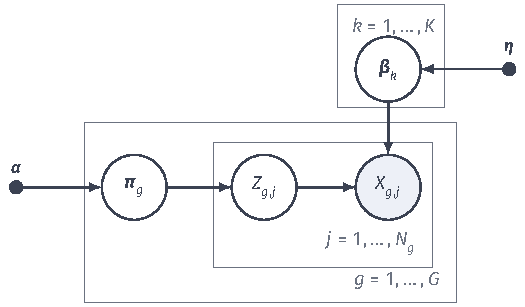
\includegraphics[width=\linewidth]{figures/03-models/03-probabilistic-graphical-models/tikz/pgm-static-directed-plates/figure.pdf}
  \caption{主题词分布也带先验的LDA板图。空心圆为随机潜在量，填色圆为观测词，实点为给定超参数。$G$个文档分别有主题比例$\bm{\pi}_g$，每篇有$N_g$个主题分配和词；$K$个主题词分布$\bm{\beta}_k$在所有文档间共享。指向词的主题参数边表示按$Z_{g,j}$选择对应分布。}
  \label{fig:pgm-static-directed-plates}
\end{figure}

模型特有的后验计算可以接回前面的通用工具。固定$\bm{\beta}_{1:K}$时，采用$q(\bm{\pi}_g)\prod_jq(Z_{g,j})$的平均场近似，令$q(\bm{\pi}_g)=\operatorname{Dirichlet}(\bm{\gamma}_g)$、$q(Z_{g,j}=k)=\rho_{g,j,k}$，其坐标更新为
\begin{equation}
  \label{eq:pgm-static-directed-lda-vi}
  \begin{aligned}
    \rho_{g,j,k}&\propto
      \beta_{k,x_{g,j}}
       \exp\!\left\{\psi(\gamma_{g,k})
                   -\psi\!\left(\sum_\ell\gamma_{g,\ell}\right)\right\},\\
    \gamma_{g,k}&=\alpha_k+\sum_j\rho_{g,j,k}.
  \end{aligned}
\end{equation}
这里$\psi(u)=d\log\Gamma(u)/du$为digamma函数，花括号中的量就是$q$下$\log\pi_{g,k}$的期望。$\bm{\gamma}_g$和$\bm{\rho}_g$共同组成局部变分参数$\bm{\phi}_g$。对每个词归一化$\rho$后交替更新，两式正是第~\ref{chap:pgm-variational}章坐标上升在该模型中的实例，而不是精确后验等式。固定全局参数时，一轮稠密局部更新通常需$O(K\sum_gN_g)$操作。

给$\bm{\beta}_k$也加Dirichlet先验后，可以把$\bm{\pi}_g$与$\bm{\beta}_k$积分掉，使用第~\ref{chap:pgm-sampling}章的Gibbs方法更新一个主题分配。令$n_{g,k}^{-}$为排除当前位置后的文档主题计数，$c_{k,a}^{-}$为全语料的主题词计数，$c_{k,\cdot}^{-}=\sum_a c_{k,a}^{-}$、$\eta_0=\sum_a\eta_a$，则
\begin{equation}
  \label{eq:pgm-static-directed-lda-gibbs}
  p(Z_{g,j}=k\mid\text{其余分配},\mathcal{D})
     \propto (n_{g,k}^{-}+\alpha_k)
        \frac{c_{k,x_{g,j}}^{-}+\eta_{x_{g,j}}}
             {c_{k,\cdot}^{-}+\eta_0}.
\end{equation}
第一项来自该文档对主题的后验预测，第二项来自主题对当前词的后验预测；与$k$无关的文档分母已约去。两项相乘再归一化，是积分共轭分布后得到的精确单点条件概率，但有限次采样得到的整体后验估计仍有误差，且可能混合缓慢。

将主题词参数作点估计时，变分EM在E步固定当前参数完成局部推断，随后在M步用$\rho$加权的全语料词频更新主题词概率。对$\bm{\alpha}$的M步涉及$\log\Gamma(\alpha_0)-\sum_k\log\Gamma(\alpha_k)$及各文档的$\mathbb{E}_q[\log\pi_{g,k}]$，可在正值约束下数值优化。把变分期望当作真后验期望，只能得到变分目标的性质，不能宣称观测似然按精确EM保证上升。采用贝叶斯主题参数时，所更新的是相应参数后验或变分因子，不再是同一个点估计问题；这些区别回到第~\ref{chap:pgm-parameter-learning}章的学习目标选择。

主题模型同样存在标签交换。在对主题对称的先验下，主题编号与比例坐标可以共同置换；即使通过非对称先验固定了一些编号，主题词分布也未必由有限语料唯一识别。两个主题几乎相同、文档过短或主题数过大时，分解尤其不稳定。词袋假设忽略词序，而主题比例的先验又限制组间变化；较高的似然不能证明学到了唯一、可命名的语义主题。

固定$K$要求在拟合前选定成分数。
\term{狄利克雷过程混合}（Dirichlet process mixture, DPM）改用卷一已定义的Dirichlet过程先验。
在标准Borel成分参数空间上记$G\sim\operatorname{DP}(c,H)$，
$c>0$对应卷一的总质量参数$\alpha$，$H$对应基概率测度$G_0$；
这里为避免与主题参数混用而更换符号。
有限分割定义见
\BookSectionRef{sec:rv-random-generation}{第一卷“数学准备”的随机概率测度与Dirichlet过程小节}。

用于混合计算的可数离散表示来自Dirichlet过程的折棒构造定理。
取相互独立的$v_k\sim\operatorname{Beta}(1,c)$与$\bm{\xi}_k\sim H$，令
\[
  w_k=v_k\prod_{\ell<k}(1-v_\ell),\qquad
  G=\sum_{k=1}^{\infty}w_k\delta_{\bm{\xi}_k}.
\]
其中$\delta_{\bm{\xi}_k}$为点质量。该构造的分布满足卷一的全部有限分割规律；
权重和为$1$只证明它是概率测度，不能单独证明它具有Dirichlet过程分布。
这里采用该构造定理，相关表述见Teh等的论述\scite{pgm-static-directed-teh2006}
再条件独立地取$\bm\zeta_j\mid G\sim G$、$\bm X_j\mid\bm\zeta_j\sim p(\cdot\mid\bm\zeta_j)$，
重复抽到同一原子意味着共享成分。随机混合测度离散不要求观测分布也离散。

给定$n$个潜在成分参数后，在任一有限分割上，Dirichlet共轭更新把分割计数加到先验参数。
由所有分割的同一更新得到
\[
  G\mid\bm\zeta_{1:n}\sim\operatorname{DP}
    \left(c+n,\frac{cH+\sum_{j=1}^n\delta_{\bm\zeta_j}}{c+n}\right).
\]
其后验均值给出下一成分参数的预测分布。

在$H$无原子时，将$G$积分掉，给定前$n$个潜在成分参数，下一条记录复用已有成分$k$的概率为$n_k/(n+c)$，抽取新成分的总概率为$c/(n+c)$。例如已有占用数为$(3,1)$且$c=1$，三个选择的概率为$0.6,0.2,0.2$。这是给定潜在分配后的先验预测；若下一条记录的观测值也已给出，还要分别乘成分预测密度与基准预测密度，再归一化。有限$n$最多占用$n$个成分；其先验期望为$\sum_{j=1}^{n}c/(c+j-1)$，因为第$j$次抽样新增成分的概率就是该和的第$j$项。“无限”放宽的是候选模型容量，不是要求实际计算无限个成分，也不是保证恢复某个真实有限类别数。

多个组需要共同使用这些候选成分时，分别从同一个连续$H$抽取独立Dirichlet过程还不够：不同组的原子几乎必然不同，不能精确共享成分。\term{层次狄利克雷过程}（hierarchical Dirichlet process, HDP）改用一个离散的随机基准分布：
\begin{equation}
  \label{eq:pgm-static-directed-hdp}
  G_0\sim\operatorname{DP}(\gamma,H),\qquad
  G_g\mid G_0\sim\operatorname{DP}(c,G_0).
\end{equation}
由于$G_0$几乎必然离散，各$G_g$的原子来自同一个可数集合，但组级权重可以不同。用于主题建模时，原子是主题词分布，文档的每个词选择一个共享主题，文档之间又有不同偏好。这同时具有层次共享、混合成员和非固定成分数量，而不是在三者之间择一。DP的离散构造及HDP如何通过随机基准共享原子，可参看Teh等人的系统论述\scite{pgm-static-directed-teh2006}

DPM与HDP把“选择一个固定$K$”转化为对分配、权重和超参数的联合推断，计算负担并未消失。截断变分方法用有限候选集近似无限模型，采样方法可以动态增删已占用成分；二者分别需要检查截断误差或链的混合。HDP还要处理组内成分与全局共享成分的关系，不能只在各组独立运行有限混合EM。浓度参数仍控制分组倾向，超参数估计与预测检验仍然必要。随机原子的编号也不赋予语义可识别性；实际应报告预测、占用成分和组间共享的不确定性，而不是只给一个未经验证的“自动主题数”。

\section{模型比较}
\label{sec:pgm-static-directed-comparison}

比较这些模型前，应固定要回答的查询。下表中的“观测似然”指给定全局参数或超参数后，对模型规定的局部潜变量完成边缘化的$p(\bm{x})$，不是再对所有未知参数积分得到的模型证据。NB与TAN按完整训练记录$(y,\bm{x})$比较，分类查询则把$Y$当作未知量。表~\ref{tab:pgm-static-directed-comparison}同时列出独立性、共享方式与非唯一性，以免把“潜变量存在”和“后验必然难算”混为一谈。

\begin{table*}[htbp]
  \centering
  \small
  \begin{tabularx}{\linewidth}{@{}
    >{\raggedright\arraybackslash}p{28mm}
    >{\raggedright\arraybackslash}p{30mm}
    >{\raggedright\arraybackslash}p{27mm}
    >{\raggedright\arraybackslash}p{30mm}
    >{\raggedright\arraybackslash}X@{}}
    \toprule
    模型与潜在量 & 独立性与共享 & 观测似然 & 局部后验 & 非唯一性与主要代价\\
    \midrule
    NB／TAN：训练时无潜变量 &
    类内独立／类内树；参数跨样本共享 &
    完整记录直接乘积 &
    类别后验枚举$K$项 &
    支持不足的条件表不确定；TAN还需选择树\\
    自回归：无随机潜变量 &
    顺序父集；条件网络可共享参数 &
    条件密度直接乘积 &
    前缀续写直接；任意补全未必易算 &
    网络参数可不唯一；优化、顺序选择与串行生成\\
    有限混合：离散分配 &
    样本在固定参数下独立；类内结构由成分决定 &
    $K$项有限和 &
    成分责任度精确 &
    标签交换、冗余成分；局部极值与退化\\
    FA／PPCA：连续因子 &
    给定因子后观测独立；共享载荷 &
    解析高斯密度 &
    解析高斯后验与缺失预测 &
    旋转及可能的额外分解歧义；维数与噪声假设\\
    LDA：连续比例与离散主题 &
    组级比例、全局主题；组内条件独立 &
    需积分比例，通常近似 &
    联合后验通常近似，局部条件可解析 &
    主题置换与重叠；局部推断和全局学习交替\\
    DPM／HDP：分配与随机测度 &
    可数候选成分；HDP跨组共享原子 &
    对未知随机量积分通常需近似 &
    采样或截断变分 &
    成分编号不唯一；占用数、超参数与近似误差\\
    \bottomrule
  \end{tabularx}
  \caption{静态有向模型的查询与计算比较。“精确”均指所述固定参数设定下的局部计算，不意味着参数已知、学习有全局保证或模型能唯一解释数据。}
  \label{tab:pgm-static-directed-comparison}
\end{table*}

直接分解把联合建模转化为局部条件分布的拟合。NB用强独立性节省样本，TAN增加少量结构搜索，自回归网络则把更多表达负担交给参数共享与非线性优化。它们避免的是完整观测似然中的潜变量求和或积分；顺序采样、任意缺失查询和条件模型失配仍可能成为瓶颈。潜变量模型也不都需要近似推断：有限混合的有限和、线性高斯模型的解析积分，都能同时给出精确似然与局部后验。

组级共享改变了推断问题的规模。pLSA在固定文档比例下只有逐词有限和；LDA把比例作为共同随机量后，同一文档的主题后验相互联系；再给主题分布加先验，又联系起不同文档。HDP进一步让候选成分数量参与推断。因此层次模型的计算困难不只来自单个潜变量取值空间大，也来自多个局部未知量必须共同解释共享观测。

这些属性可以组合。例如混合因子分析先选离散成分，再用该成分的连续因子生成观测；每个成分边缘化后仍是一个低秩加对角协方差的高斯，责任度与因子后验都可解析计算。自回归条件也可以用有限混合参数化，组级载荷可以再设置层次先验。是否采用离散潜变量、是否线性高斯、是否跨组共享、是否逐项生成，应按不同维度分别回答，而不根据一个模型名称一次决定。

可识别性则约束结果能怎样解释。给定充分数据，条件概率或观测协方差可能估计得很准确，但这不自动识别网络的每个权重、混合的编号或因子的方向。模型选择应结合留出预测与建模目标：若要解释潜在结构，还需报告这些对称性及稳定性；若主要用于补全，则应检验条件预测与不确定性，而不是只比较完整记录的似然。计算可行、预测有效和潜在解释可信，是需要分别验证的三项判断。

\section{本章小结}
\label{sec:pgm-static-directed-summary}

静态有向模型用局部条件分布定义联合分布，但观测分布可以来自两种不同计算过程：直接评价全部观测节点的分解，或在更大的联合分布中消去潜变量。两个传感器的例子说明，同一张观测概率表既可以写成自回归条件，也可以写成隐藏类别的混合；前者给出预测顺序，后者提供一个需要另行验证的潜在解释。

潜变量改变的不只是模型图形。有限混合把学习变成责任度与成分参数的交替估计，却保留精确的局部后验；线性高斯模型用解析积分连接协方差、降维表示和缺失预测；层次结构与混合成员把多个样本或组的未知量联系起来，常使联合后验需要近似计算。离散或连续描述潜变量的取值，层次或混合成员描述共享方式，二者可以共同出现。标签交换、旋转和冗余分解进一步表明，观测分布的确定性不等于潜在坐标的唯一性。

面对一个新模型，应检查它如何归一化、目标查询需要消去哪些变量、哪些量在数据之间共享，以及参数估计是否受到退化或非唯一性的影响。接下来的第~\ref{chap:pgm-energy-models}章改用对称相互作用组织模型，比较联合归一化与只对输出归一化的差别。神经参数化不会取消这些概率问题；第~\ref{chap:pgm-generative}章再以本章的自回归分解和高斯潜变量模型为参照，比较更灵活的密度构造。
